\documentclass[10pt,aspectratio=169]{beamer}

% ============== THEME ==============
\usetheme{metropolis}
\usepackage[T1]{fontenc}
\usepackage[utf8]{inputenc}
\usepackage{appendixnumberbeamer}
\usepackage{booktabs}
\usepackage{tabularx}
\usepackage{array}
\usepackage{colortbl}
\providecommand{\citep}[1]{}
\providecommand{\cite}[1]{}
\usepackage{xcolor}
\usepackage{tikz}
\usepackage{pgfplots}
\pgfplotsset{compat=1.17}

% ============== COLORS ==============
\definecolor{ubblue}{HTML}{1F3A93}
\definecolor{ubaccent}{HTML}{C0392B}
\definecolor{ubsoft}{HTML}{ECF0F1}
\definecolor{ubdark}{HTML}{2C3E50}
\definecolor{ubgreen}{HTML}{27AE60}
\definecolor{uborange}{HTML}{E67E22}

\setbeamercolor{normal text}{fg=ubdark}
\setbeamercolor{alerted text}{fg=ubaccent}
\setbeamercolor{example text}{fg=ubgreen}
\setbeamercolor{progress bar}{fg=ubaccent}
\setbeamercolor{title separator}{fg=ubaccent}
\setbeamercolor{frametitle}{bg=ubblue,fg=white}
\setbeamercolor{block title}{bg=ubblue!15,fg=ubblue}
\setbeamercolor{block body}{bg=ubblue!5,fg=ubdark}

\metroset{block=fill, progressbar=frametitle, sectionpage=progressbar, numbering=fraction}

% ============== TITLE ==============
\title{\textbf{Detectia limbajului ofensiv, urii\\ si misoginiei in texte romanesti}}
\subtitle{Pipeline unificat cu cinci clase: TF-IDF baselines si RoBERT}
\date{\today}
\author{Adrian Aparaschivei \and Roberta-Gabriela Nechita \\ Bianca-Nicoleta Paraschiv \and El-Abassi Tamer Alexandru}
\institute{Universitatea din Bucuresti --- Facultatea de Matematica si Informatica}

% ============== HELPERS ==============
\newcommand{\bignum}[1]{{\fontsize{34}{40}\selectfont\textbf{\textcolor{ubaccent}{#1}}}}
\newcommand{\sub}[1]{{\small\textcolor{ubdark!70}{#1}}}
\newcommand{\contribcard}[2]{%
  \begin{minipage}[t][2.4cm][t]{0.46\textwidth}%
    \begin{beamercolorbox}[wd=\linewidth,ht=2.4cm,dp=0pt,rounded=true,shadow=true,sep=8pt]{block body}%
      \parbox[t][2.0cm][t]{0.94\linewidth}{%
        \textbf{\textcolor{ubblue}{#1}}\\[0.4em]%
        \footnotesize #2%
      }%
    \end{beamercolorbox}%
  \end{minipage}%
}

\begin{document}

% ====================================================
\maketitle
% ====================================================

\begin{frame}{Cuprins}
\vspace{0.4em}
\newcommand{\tocitem}[2]{%
  \makebox[0.7cm][l]{\textcolor{ubaccent}{\textbf{\large#1.}}}\large#2\\[0.55em]}
\begin{columns}[T,onlytextwidth]
  \column{0.48\textwidth}
  \tocitem{1}{Motivatie}
  \tocitem{2}{Related Work}
  \tocitem{3}{Date}
  \tocitem{4}{Preprocesare}
  \column{0.48\textwidth}
  \tocitem{5}{Modele}
  \tocitem{6}{Rezultate}
  \tocitem{7}{Perspective}
  \tocitem{8}{Concluzii}
\end{columns}
\end{frame}

% ====================================================
\section{Motivatie}
% ====================================================

\begin{frame}{De ce hate speech in romana?}
\begin{columns}[T,onlytextwidth]
\column{0.5\textwidth}
\begin{itemize}
  \setlength\itemsep{0.7em}
  \item \textbf{Limba cu putine resurse} \\ \sub{putine corpusuri publice de hate speech}
  \item \textbf{Text social zgomotos} \\ \sub{diacritice lipsa, slang, leetspeak}
  \item \textbf{Dezechilibru sever de clase} \\ \sub{rasism + homofobie $<$ 1\%}
  \item \textbf{Sens dependent de context} \\ \sub{insulta vs. citat vs. critica}
\end{itemize}
\column{0.5\textwidth}
\begin{block}{Capcana acuratetei}
Un model care prezice \emph{mereu} \\ \textit{non-offensive} atinge\\[0.3em]
\centering\bignum{78\%}\\[0.2em]
\sub{accuracy --- dar nu detecteaza nimic.}
\end{block}
\vspace{0.3em}
\centering \alert{$\Rightarrow$ macro-F1 este metrica corecta.}
\end{columns}
\end{frame}

\begin{frame}{Contributiile pe scurt}
\vspace{0.4em}
\begin{center}
\contribcard{Corpus unificat}{%
  \textsc{news-ro-offense} $\cup$ CoRoSeOf \\
  $\rightarrow$ \textbf{43{,}061} exemple, 5 clase}\hspace{0.04\textwidth}%
\contribcard{Comparatie controlata}{%
  LogReg vs.\ Calibrated Linear SVM \\
  \sub{TF-IDF word+char comun, + RoBERT}}

\vspace{0.7em}

\contribcard{Preprocesare adaptata romanei}{%
  diacritice, leetspeak, stemming,\\
  emoji, stopwords cu negatii}\hspace{0.04\textwidth}%
\contribcard{Ablatie si error analysis}{%
  Ce influenteaza macro-F1\\
  + unde gresesc modelele}
\end{center}
\end{frame}

% ====================================================
\section{Related Work}
% ====================================================

\begin{frame}{Peisajul domeniului}
\begin{columns}[T]
\column{0.55\textwidth}
\begin{itemize}
  \setlength\itemsep{0.7em}
  \item \textbf{OffensEval 2019/2020} \\ \sub{taxonomie ierarhica, multilingv}
  \item \textbf{HatEval 2019} \\ \sub{ura impotriva femeilor si imigrantilor}
  \item \textbf{Survey-uri} \sub{(Fortuna \& Nunes 2018; Schmidt \& Wiegand 2017)}
  \item \textbf{Modele perspective-aware} \\ \sub{(Akhtar et al., 2021)}
\end{itemize}
\column{0.45\textwidth}
\begin{alertblock}{Idee cheie \sub{(Akhtar et al., 2021)}}
Dezacordul intre adnotatori este \emph{semnal}, nu zgomot.\\[0.3em]
\sub{$\Rightarrow$ separam abuzul targetat pe identitate de insulta generica.}
\end{alertblock}
\end{columns}
\end{frame}

% ====================================================
\section{Date}
% ====================================================

\begin{frame}{Doua surse complementare}
\centering
\renewcommand{\arraystretch}{1.3}
\begin{tabular}{lrl}
\toprule
\textbf{Sursa} & \textbf{Randuri} & \textbf{Rol} \\
\midrule
CoRoSeOf            & 39{,}008 & sexism / ofensa \\
\textsc{news-ro-offense} &  4{,}053 & 5-class hate / offense \\
\midrule
\textbf{Unificat}   & \textbf{43{,}061} & schema comuna \\
\bottomrule
\end{tabular}
\vspace{1em}
\begin{block}{Schema}
\texttt{text} $\cdot$ \texttt{label\_5} $\cdot$ \texttt{offensive\_flag} $\cdot$ \texttt{sexism\_flag} $\cdot$ \texttt{target} $\cdot$ \texttt{sexism\_subtype} $\cdot$ \texttt{quality}
\end{block}
\end{frame}

\begin{frame}{Taxonomia cu cinci clase}
\vspace{0.5em}
\begin{center}
\renewcommand{\arraystretch}{1.35}
\begin{tabular}{cll}
\toprule
\textbf{ID} & \textbf{Clasa} & \textbf{Semnificatie} \\
\midrule
0 & \textsc{non-off.}      & text neofensiv \\
1 & \textsc{insult}        & insulta generica \\
2 & \textsc{racism}        & continut rasist \\
3 & \textsc{homophobia}    & continut homofob \\
4 & \textsc{sexism}        & sexism / misoginie \\
\bottomrule
\end{tabular}
\end{center}
\vspace{0.6em}
\begin{center}
\begin{minipage}{0.85\textwidth}
\centering\sub{Maparea pastreaza subtipurile CoRoSeOf\\ (\textit{direct, descriptive, reporting}) in \texttt{sexism\_subtype}.}
\end{minipage}
\end{center}
\end{frame}

\begin{frame}{Distributia: o coada lunga de ura}
\vspace{0.4em}
\begin{columns}[c,onlytextwidth]
\column{0.68\textwidth}
\centering
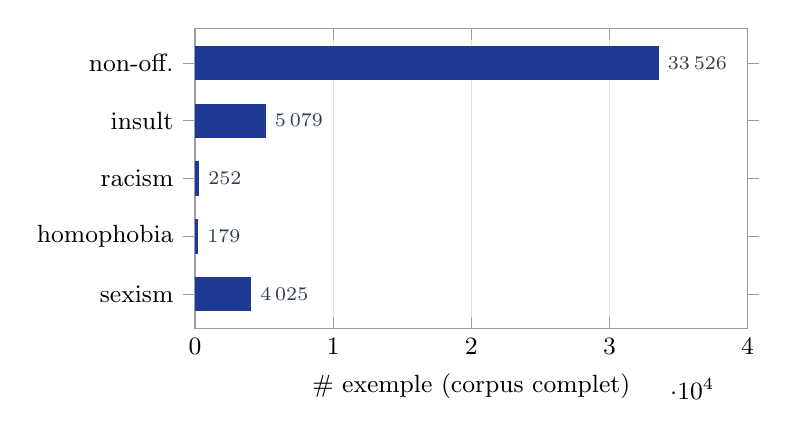
\begin{tikzpicture}
\begin{axis}[
    width=8.6cm, height=5.4cm,
    xbar, bar width=12pt,
    xmin=0, xmax=40000,
    xlabel={\small \# exemple (corpus complet)},
    symbolic y coords={sexism,homophobia,racism,insult,non-off.},
    ytick=data,
    nodes near coords={\pgfmathprintnumber[1000 sep={\,},fixed,precision=0]\pgfplotspointmeta},
    every node near coord/.append style={font=\scriptsize, color=ubdark, anchor=west},
    enlarge y limits=0.15,
    tick label style={font=\small},
    axis line style={ubdark!50},
    tick style={ubdark!50},
    xmajorgrids=true, grid style={ubdark!15},
]
\addplot+[fill=ubblue,draw=ubblue] coordinates {
    (33526,non-off.) (5079,insult) (252,racism) (179,homophobia) (4025,sexism)
};
\end{axis}
\end{tikzpicture}
\column{0.32\textwidth}
\begin{alertblock}{Long tail}
\bignum{$\approx$\,1\%}\\[0.3em]
\sub{Rasism + homofobie\\ din intregul corpus.}
\end{alertblock}
\vspace{0.4em}
\sub{Non-offensive domina; clasele de ura targetata sunt extrem de rare.}
\end{columns}
\end{frame}

\begin{frame}{Subset experimental stratificat}
\vspace{0.3em}
\begin{columns}[T,onlytextwidth]
\column{0.46\textwidth}
\begin{block}{Compozitie}
\small
\begin{itemize}\setlength\itemsep{0.25em}
  \item \textbf{800} non-off. \sub{(seed=42)}
  \item \textbf{200} insult \quad \textbf{200} sexism
  \item \textbf{toate} racism \sub{(252)}
  \item \textbf{toate} homophobia \sub{(179)}
\end{itemize}
\end{block}
\vspace{0.4em}
\begin{center}
\bignum{1{,}631}\\[-0.2em]
\sub{randuri total --- 800 non-off / 831 ofensive}
\end{center}

\column{0.5\textwidth}
\begin{block}{Split stratificat 70 / 15 / 15}
\centering
\renewcommand{\arraystretch}{1.25}
\footnotesize
\begin{tabular}{lrrrrrr}
\toprule
\textbf{Split} & \textbf{N} & 0 & 1 & 2 & 3 & 4 \\
\midrule
Train & 1{,}141 & 560 & 140 & 176 & 125 & 140 \\
Val   &   245   & 120 &  30 &  38 &  27 &  30 \\
Test  &   245   & 120 &  30 &  38 &  27 &  30 \\
\bottomrule
\end{tabular}
\end{block}
\vspace{0.3em}
\begin{center}\sub{Stratificare per-clasa $\Rightarrow$ fiecare clasa apare in fiecare partitie.}\end{center}
\end{columns}
\end{frame}

% ====================================================
\section{Preprocesare}
% ====================================================

\begin{frame}{Preprocesare adaptata romanei}
\begin{columns}[T,onlytextwidth]
\column{0.5\textwidth}
\textbf{Pipeline}
\begin{itemize}
  \setlength\itemsep{0.4em}
  \item URLs $\to$ \texttt{<URL>}, mentions $\to$ \texttt{<USER>}
  \item Hashtag splitting
  \item Emoji $\to$ text \sub{(semnal afectiv)}
  \item Colaps de elongatii \\ \sub{\textit{frumoasaaaa} $\to$ \textit{frumoasaa}}
  \item Lowercase + scoatere diacritice
  \item \alert{Leetspeak} \sub{\texttt{0$\to$o, 3$\to$e, 4$\to$a, @$\to$a}}
  \item Stopwords \emph{mai putin} \textit{nu, nici, fara}
  \item \alert{Stemming} \sub{morfologie bogata}
\end{itemize}
\column{0.5\textwidth}
\begin{exampleblock}{Exemplu pas cu pas}
\footnotesize
\begin{tabularx}{\linewidth}{@{}lX@{}}
\textbf{Brut}        & \textit{@user esti pr0asta!! \#romani} \\
mention/hashtag      & \texttt{<USER> esti pr0asta romani} \\
leetspeak            & \texttt{<USER> esti proasta romani} \\
lowercase            & \texttt{<user> esti proasta romani} \\
stopwords            & \texttt{<user> proasta romani} \\
\end{tabularx}
\end{exampleblock}
\vspace{0.3em}
\centering \alert{130k $\to$ 12.7k} features dupa stemming.
\end{columns}
\end{frame}

% ====================================================
\section{Modele}
% ====================================================

\begin{frame}{Spatiu de features comun}
\begin{block}{TF-IDF: word + character}
\centering
word $(1,2)$-grams \quad $\oplus$ \quad char $(3,5)$-grams\\[0.3em]
\sub{\texttt{min\_df=3, max\_df=0.9, sublinear\_tf=True}} \\[0.2em]
$\approx$ \textbf{20{,}000} features (subset demo)
\end{block}
\vspace{0.6em}
\centering Acelasi vectorizer, fit doar pe \emph{train} $\Rightarrow$ \alert{diferentele vin din clasificator.}
\end{frame}

\begin{frame}{Trei clasificatori, un singur feature space}
\begin{columns}[T,onlytextwidth]
\column{0.33\textwidth}
\begin{block}{LogReg}
\small
softmax posterior \\
$C \in \{10^{-3},\dots,10^{2}\}$ \\
\textbf{best $C=0.3$} \\
\texttt{class\_weight=balanced} \\
\alert{stem=True}
\end{block}
\column{0.33\textwidth}
\begin{block}{Linear SVM}
\small
max-margin hyperplane \\
$C \in \{0.1,\dots,5.0\}$ \\
\textbf{best $C=0.5$} \\
+ \alert{Platt calibration} (5-fold) \\
stem=False
\end{block}
\column{0.33\textwidth}
\begin{block}{RoBERT}
\small
Romanian BERT \\
AdamW, lr $=2\!\cdot\!10^{-5}$ \\
batch 16, 5 epochs \\
classifier head $\to$ 5 clase \\
\sub{baseline contextual}
\end{block}
\end{columns}
\vspace{0.6em}
\centering 5-fold \texttt{StratifiedKFold} CV --- evita fold-uri fara homophobia (doar 125 ex.\ train).
\end{frame}

% ====================================================
\section{Rezultate}
% ====================================================

\begin{frame}{Cifrele principale}
\centering
\renewcommand{\arraystretch}{1.4}
\begin{tabular}{lcccccc}
\toprule
\textbf{Model} & \textbf{Acc.} & \textbf{F1\textsubscript{macro}} & F1\textsubscript{ins.} & F1\textsubscript{rac.} & F1\textsubscript{hom.} & F1\textsubscript{sex.} \\
\midrule
LogReg     & 0.751 & 0.698 & 0.517 & 0.784 & 0.667 & 0.690 \\
\rowcolor{ubblue!10}
\textbf{Linear SVM} & \textbf{0.788} & \textbf{0.720} & 0.490 & \textbf{0.833} & 0.640 & \textbf{0.772} \\
\bottomrule
\end{tabular}
\vspace{1em}

\begin{columns}[T]
\column{0.5\textwidth}
\centering \bignum{+0.022} \\ \sub{macro-F1, SVM peste LogReg}
\column{0.5\textwidth}
\centering \bignum{+0.082} \\ \sub{F1 pe \textit{sexism}, SVM peste LogReg}
\end{columns}
\end{frame}

\begin{frame}{Macro-F1 pe clase}
\centering
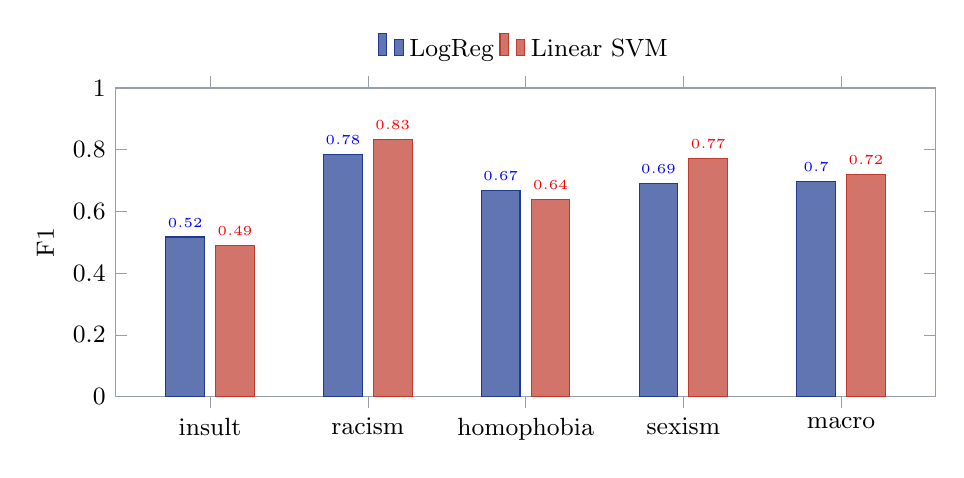
\begin{tikzpicture}
\begin{axis}[
    width=12cm, height=5.5cm,
    ybar=4pt, bar width=14pt,
    ymin=0, ymax=1.0,
    ylabel={\small F1},
    symbolic x coords={insult,racism,homophobia,sexism,macro},
    xtick=data,
    legend style={at={(0.5,1.05)},anchor=south,legend columns=2,draw=none,font=\small},
    enlarge x limits=0.15,
    nodes near coords, nodes near coords style={font=\tiny,rotate=0,/pgf/number format/.cd,fixed,precision=2},
    tick label style={font=\small},
    axis line style={ubdark!50}, tick style={ubdark!50},
]
\addplot+[fill=ubblue!70,draw=ubblue] coordinates {
    (insult,0.517) (racism,0.784) (homophobia,0.667) (sexism,0.690) (macro,0.698)};
\addplot+[fill=ubaccent!70,draw=ubaccent] coordinates {
    (insult,0.490) (racism,0.833) (homophobia,0.640) (sexism,0.772) (macro,0.720)};
\legend{LogReg, Linear SVM}
\end{axis}
\end{tikzpicture}

\vspace{0.4em}
\begin{center}
\begin{minipage}{0.85\textwidth}
\centering\alert{SVM castiga pe clasele minoritare; \textit{insult} ramane cea mai grea.}
\end{minipage}
\end{center}
\end{frame}

\begin{frame}{Ablatie --- ce a contat de fapt?}
\centering
\renewcommand{\arraystretch}{1.3}
\begin{tabular}{lcc}
\toprule
\textbf{Modificare (LogReg)} & \textbf{Macro-F1} & \textbf{$\Delta$} \\
\midrule
Baseline                                & 0.671 & --- \\
\rowcolor{ubgreen!10}
+ Stemming \sub{(130k $\to$ 12.7k feats.)} & 0.691 & \textcolor{ubgreen}{+0.020} \\
+ \texttt{min\_df=3, max\_df=0.9}        & 0.698 & \textcolor{ubgreen}{+0.007} \\
+ char $(3,5)$ vs.\ $(2,4)/(3,6)$        & 0.698 & cea mai buna \\
\midrule
\textbf{Final}                          & \textbf{0.698} & \\
\bottomrule
\end{tabular}

\vspace{0.8em}
\begin{center}
\begin{minipage}{0.88\textwidth}
\centering\sub{Pentru SVM: vectorizer comun word+char + Platt calibration + \texttt{dual=auto} $\Rightarrow$ 0.645 $\to$ \textbf{0.720}.}
\end{minipage}
\end{center}
\end{frame}

\begin{frame}{Unde gresesc inca modelele}
\begin{columns}[T,onlytextwidth]
\column{0.55\textwidth}
\begin{itemize}
  \setlength\itemsep{0.6em}
  \item \alert{insult $\leftrightarrow$ sexism} \\ \sub{granita dependenta de adnotare}
  \item \textbf{homophobia} cea mai grea \\ \sub{doar 125 exemple train}
  \item \textbf{Mentiune neutra $\to$ non-off.} \\ \sub{lipseste contextul pragmatic}
\end{itemize}
\column{0.45\textwidth}
\begin{alertblock}{Pattern}
Bottleneck-ul nu mai este \\\emph{modelul} --- ci \emph{datele}.\\[0.3em]
\sub{Clasele rare au $<$ 40 ex.\ pe dev; o singura greseala muta F1 cu cateva puncte.}
\end{alertblock}
\end{columns}
\end{frame}

% ====================================================
\section{Perspective}
% ====================================================

\begin{frame}{Future work}
\begin{itemize}
  \setlength\itemsep{0.8em}
  \item \textbf{Extinderea claselor rare} \\ \sub{adnotare targetata pentru racism si homophobia}
  \item \textbf{Cross-lingual transfer} \\ \sub{folosirea corpusurilor de hate speech engleze/italiene}
  \item \textbf{Modele perspective-aware} \sub{(Akhtar et al., 2021)} \\ \sub{label-uri multi-annotator, ensemble pe dezacord}
  \item \textbf{Scenariu de deployment} \\ \sub{flag-and-defer catre moderator inainte de publicare}
\end{itemize}
\end{frame}

\begin{frame}{Limitari}
\begin{columns}[T,onlytextwidth]
\column{0.5\textwidth}
\begin{itemize}
  \item \textbf{Clase rare} \\ \sub{179 ex.\ homophobia in total}
  \item \textbf{Domain mismatch} \\ \sub{stiri vs.\ text social}
  \item \textbf{Doar romana} \\ \sub{retraining necesar pentru transfer}
\end{itemize}
\column{0.5\textwidth}
\begin{itemize}
  \item \textbf{Limitarile TF-IDF} \\ \sub{rateaza sarcasm, stereotip implicit}
  \item \textbf{Subiectivitate la adnotare} \\ \sub{un singur label ascunde dezacordul}
\end{itemize}
\end{columns}
\end{frame}

\begin{frame}{Declaratie etica}
\begin{block}{}
Setul de date contine \textbf{limbaj ofensiv si potential daunator}.\\[0.4em]
Modelele propuse sunt destinate doar pentru \textbf{cercetare si asistenta la moderare}.\\[0.4em]
Orice deployment in productie necesita \alert{revizuire umana} pentru a evita decizii automate incorecte sau injuste.
\end{block}
\end{frame}

% ====================================================
\section{Concluzii}
% ====================================================

\begin{frame}{Trei idei de retinut}
\begin{enumerate}
  \setlength\itemsep{0.9em}
  \item \textbf{Unificarea conteaza.} \\ \sub{Doua corpusuri eterogene $\to$ o taxonomie utila cu 5 clase.}
  \item \textbf{SVM calibrat bate LogReg.} \\ \sub{0.720 vs.\ 0.698 macro-F1 pe acelasi feature space.}
  \item \textbf{Datele, nu modelul, sunt plafonul.} \\ \sub{Clasele minoritare misca macro-F1 --- mai multe exemple.}
\end{enumerate}
\end{frame}

% ====================================================
\begin{frame}[standout]
\centering
\Huge Multumim! \\[0.6em]
\large Intrebari?\\[1em]
\normalsize \sub{news-ro-offense $\cup$ CoRoSeOf} \quad \sub{Universitatea din Bucuresti}
\end{frame}
% ====================================================

\appendix

\begin{frame}{Referinte}
\footnotesize
\begin{thebibliography}{9}
\bibitem{akhtar2021whose} Akhtar, Basile, Patti (2021). \emph{Whose Opinions Matter? Perspective-Aware Models}. arXiv:2106.15896.
\bibitem{readerbenchNewsRoOffense} ReaderBench (2024). \emph{news-ro-offense}. Hugging Face.
\bibitem{coroseof} Hoefels (2024). \emph{CoRoSeOf}. GitHub.
\bibitem{zampieri2019offenseval} Zampieri et al.\ (2019). \emph{OffensEval (SemEval Task 6)}.
\bibitem{zampieri2020offenseval} Zampieri et al.\ (2020). \emph{Multilingual OffensEval}.
\bibitem{basile2019hateval} Basile et al.\ (2019). \emph{HatEval (SemEval Task 5)}.
\bibitem{fortuna2018survey} Fortuna \& Nunes (2018). \emph{A Survey on Automatic Detection of Hate Speech}. ACM CSUR.
\bibitem{schmidt2017survey} Schmidt \& Wiegand (2017). \emph{A Survey on Hate Speech Detection using NLP}.
\end{thebibliography}
\end{frame}

\end{document}
